\chapter{Empirical priors: pancreatitis}
\label{applications-priors_empirical}

Systematic review for the GBD 2010 Study often found a few regions for
which detailed data on the age pattern of disease were available, but
many more regions for which cases were reported with much sparser
age specificity.  Hierarchical modeling using an empirical Bayesian
prior is our way to conduct partial pooling and borrow strength from
the regions with age-specific data to produce estimates of age
patterns in regions where few or no age-specific data are
available.  This chapter demonstrates the results of partial pooling
at the regional level, where country-to-country variation is quite
pronounced, by examining the estimation of age-specific pancreatitis
incidence in Western Europe.

Pancreatitis is the inflammation of the pancreas, most commonly
caused by alcohol or gallstones.  In most cases, the disease resolves
itself and there is no need for treatment.  However, some acute
cases develop pancreatic necrosis and systemic organ failure.  These
complications require immediate treatment and have a high mortality risk.
\cite{raraty_acute_2004, banks_epidemiology_2002, sekimoto_jpn_2006}

Data from systematic review yielded $3950$ incidence data points,
$1053$ of which were from Western Europe and constitute the example
in this chapter.  As shown in figure~\ref{fig:app-pan data}, the data
from Western Europe are very heterogeneous.

    \begin{figure}[h]
        \begin{center}
            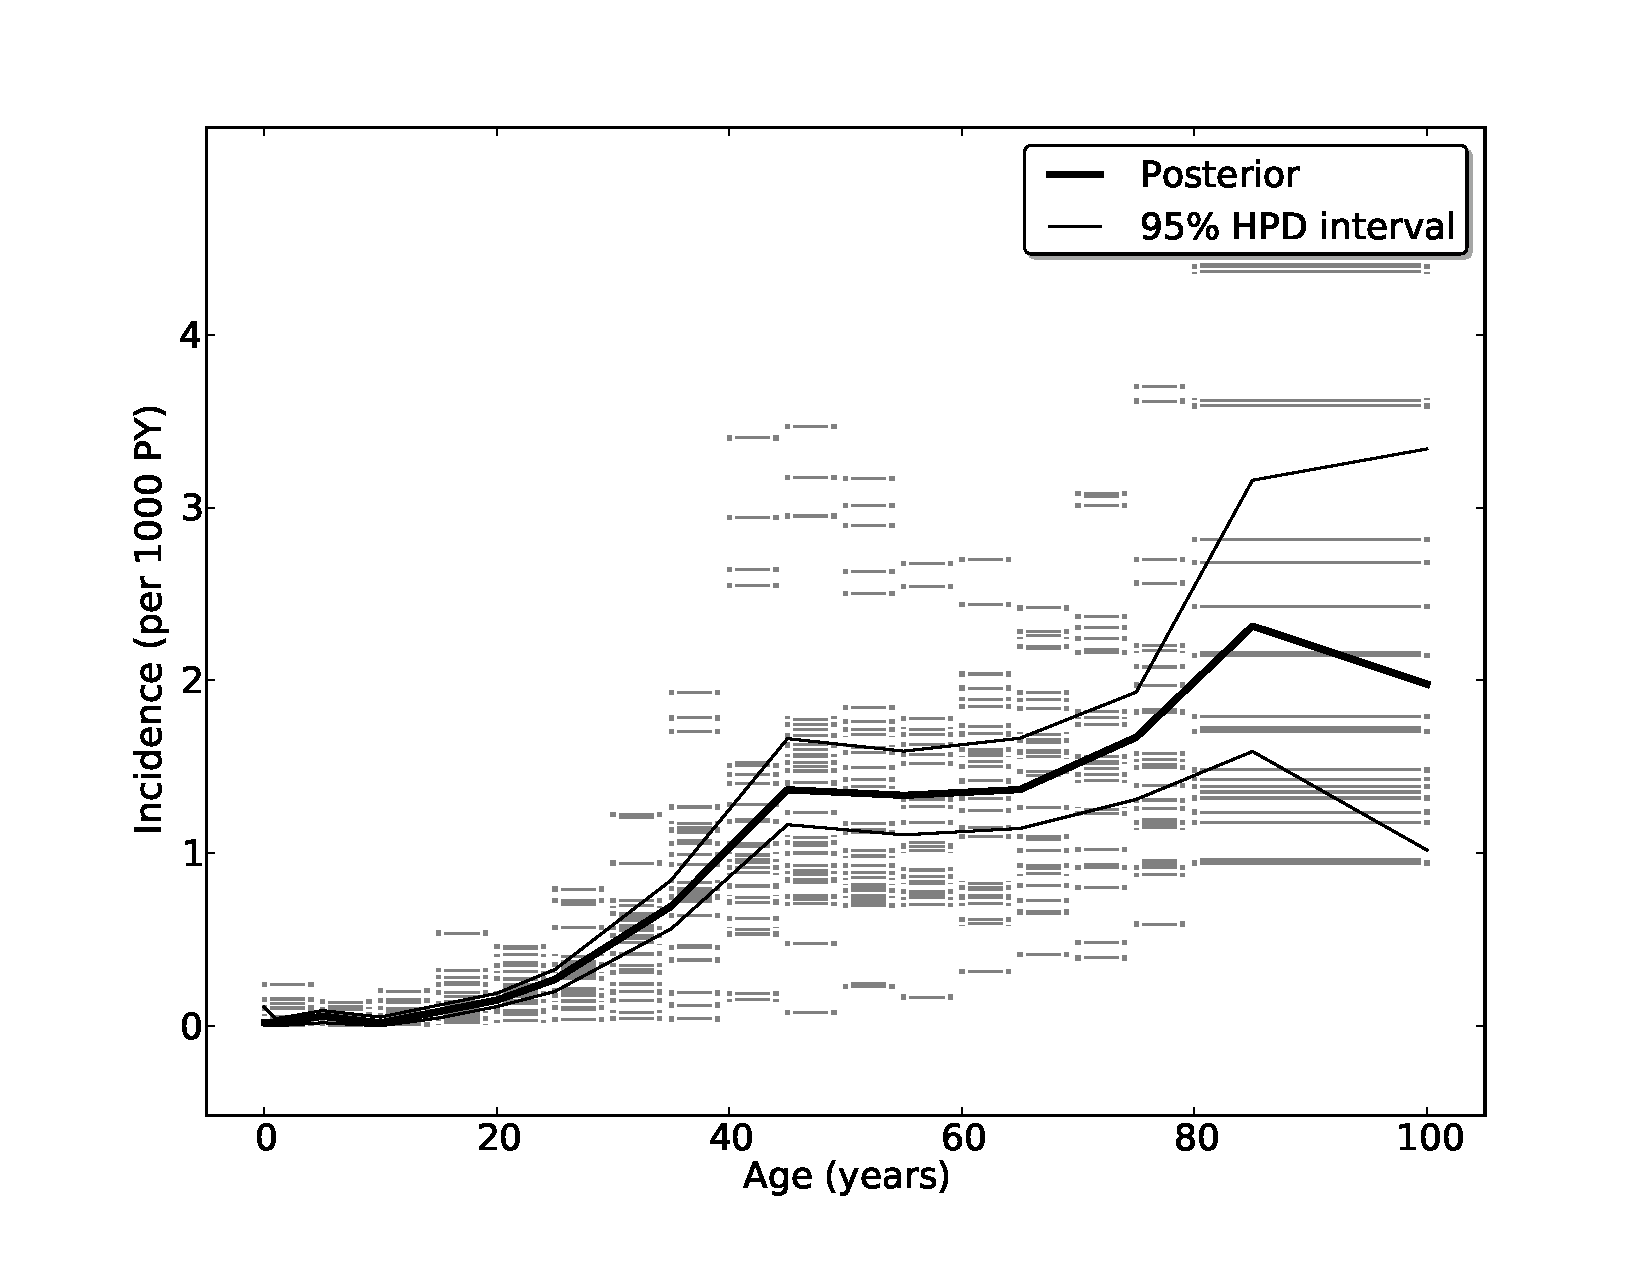
\includegraphics[width=\textwidth]{pancreatitis-we_data.pdf}
            \caption{Pancreatitis incidence data
              with pooled estimates for males and females in Western Europe in 2005.}
            \label{fig:app-pan data}
        \end{center}
    \end{figure}

Closer investigation shows that some of the heterogeneity in the data
is caused by different age patterns between countries.  Using the
pooled-data estimates from figure~\ref{fig:app-pan data} as an
empirical prior for estimates based only on country-specific data,
posterior estimates for countries with partial pooling are shown in
figure~\ref{fig:app-pan compare}.  When there are no data to say
otherwise, the posterior estimate follows the empirical prior with large
uncertainty intervals since the countries with data show a lot of
country-to-country variation (this large uncertainty is also the
reason why the means of the empirical prior and posterior estimates for Germany
in panel (d) do not match precisely).

    \begin{figure}[h]
        \begin{center}
            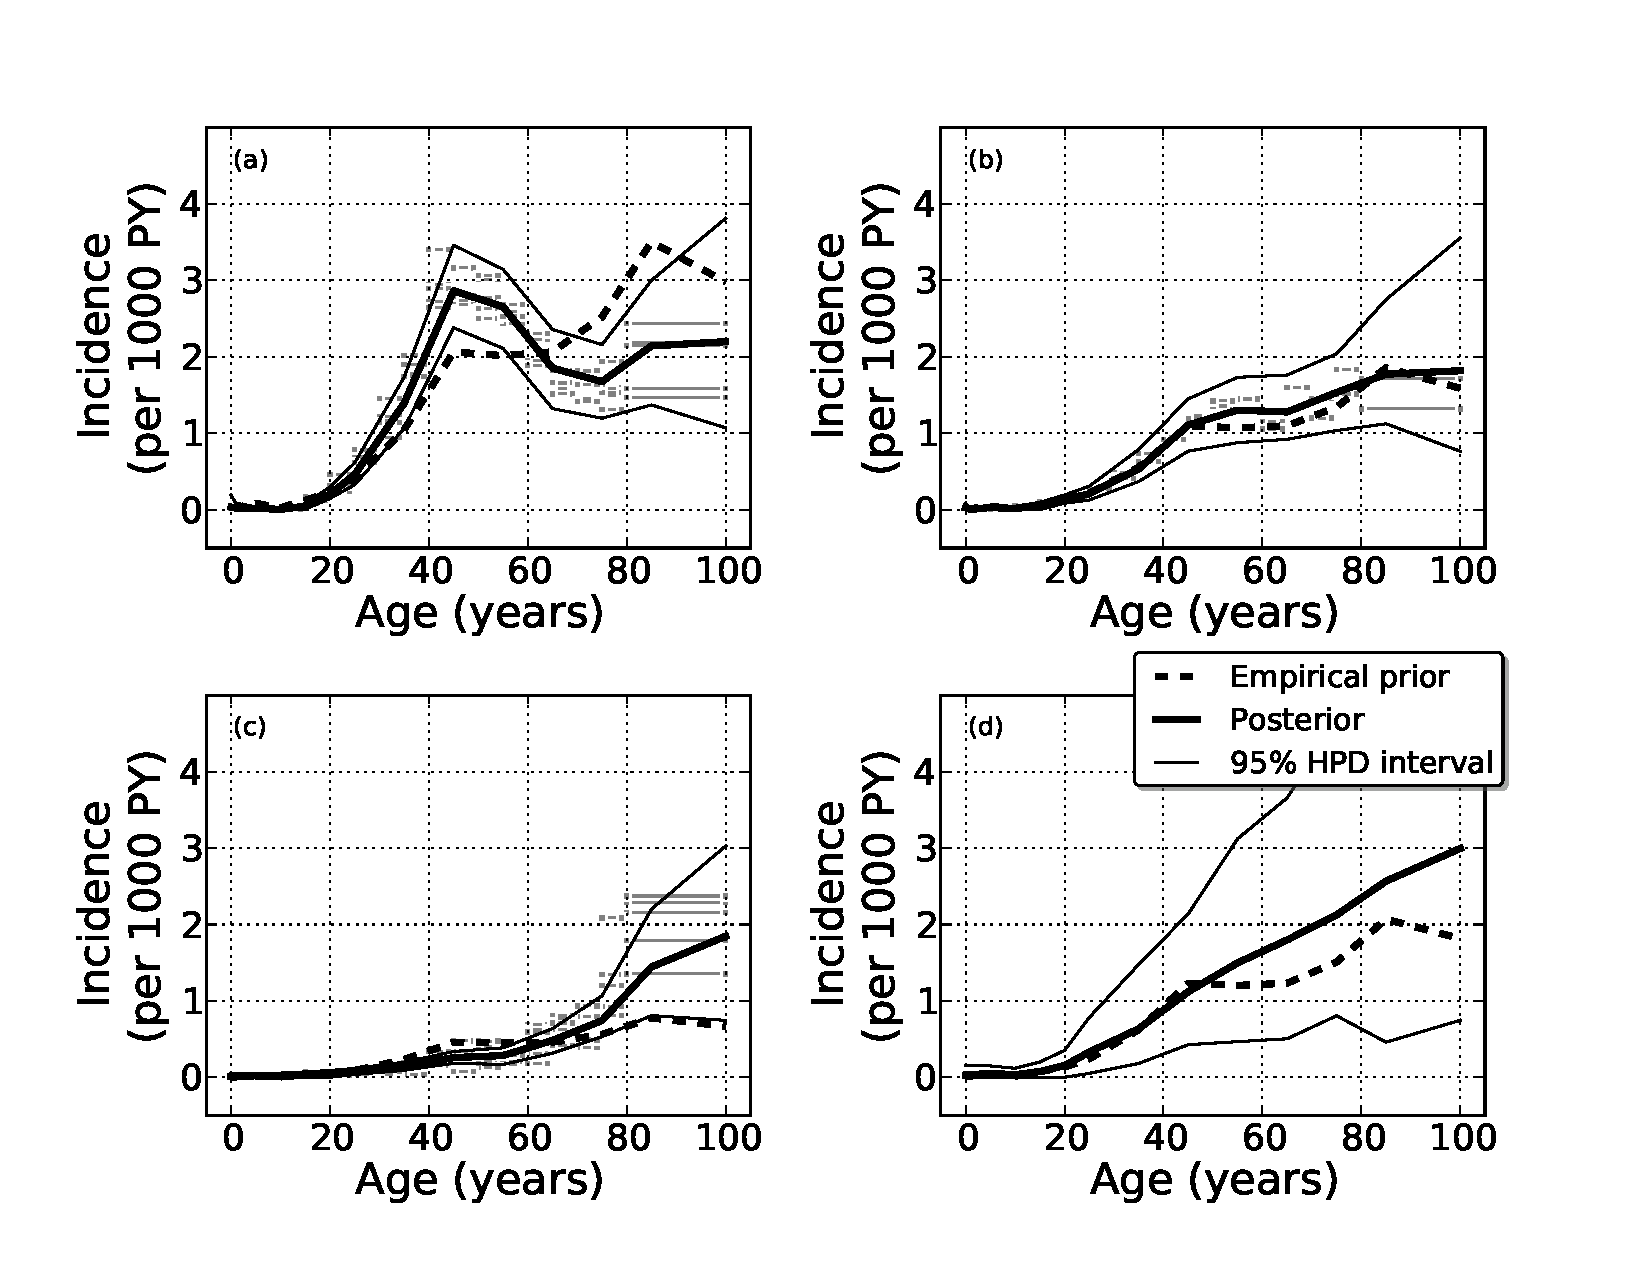
\includegraphics[width=\textwidth]{pancreatitis-we_compare.pdf}
            \caption[Comparison of pancreatitis incidence estimates
              for 2005]{Comparison of pancreatitis incidence estimates
              for 2005 for (a) Finland, (b) the Netherlands, (c)
              Cyprus, and (d) Germany.  The estimated incidence using
              pooled data from figure~\ref{fig:app-pan data} was
              applied as an empirical prior to the sex-specific
              incidence to improve estimates.}
            \label{fig:app-pan compare}
        \end{center}
    \end{figure}

Empirical priors provide data-derived relationships to guide the
modeling process.  In cases where the data are less clear, empirical
priors provide a principled and computationally tractable way to
borrow strength between regions for estimation.
